%! TEX root = dan_oyama.tex
\documentclass[../geometrymemo.tex]{subfiles}

\begin{document}
\section{Ti\textit{k}Z 入門 --- 大山 壇}
\label{sec:danoyama}

In this section, we will try some codes explained here: \url{https://note.com/dan_oyama/n/n6c3ae2a270ac}.
This is a series of explanation by 大山 壇 (Dan Oyama) a 予備校講師（数学科）.

\subsection{(2) 関数グラフを描く}

\subsubsection{座標軸}

座標軸は以下のように書いて，また原点 \(0,0\) は斜体 (italic) で書きます．
\begin{tcblisting}{title=座標軸の描き方}
    \begin{tikzpicture}[scale=1]
        \draw[->,>=stealth,semithick] (-3,0)--(3,0) node[right]{$x$}; %x軸
        \draw[->,>=stealth,semithick] (0,-1)--(0,4) node[left]{$y$}; %y軸
        \draw (0,0) node[below left]{$O$}; %原点
    \end{tikzpicture}
\end{tcblisting}

\subsubsection{関数グラフの入力}

\begin{tcblisting}{title=\texttt{plot} と \texttt{domain} を使う}
    \begin{tikzpicture}[scale=1]
        \draw[->,>=stealth,semithick] (-3,0)--(3,0) node[right]{$x$}; %x軸
        \draw[->,>=stealth,semithick] (0,-1)--(0,4) node[left]{$y$}; %y軸
        \draw (0,0) node[below left]{$O$}; %原点
        \draw[thick,domain=-3:3] plot(\x,\x/2+1);
    \end{tikzpicture}
\end{tcblisting}

\subsubsection{滑らかな曲線を描く}

\begin{tcblisting}{title=samples オプション}
    \begin{tikzpicture}[scale=1,samples=300]
        \draw[->,>=stealth,semithick] (-4,0)--(4,0) node[right]{$x$}; %x軸
        \draw[->,>=stealth,semithick] (0,-3)--(0,3) node[left]{$y$}; %y軸
        \draw (0,0) node[below left]{$O$}; %原点
        \draw[thick,domain=-4:4] plot(\x,{2*sin(\x r)});
    \end{tikzpicture}
\end{tcblisting}

\subsubsection{図を切り取る}

\lstinlineiv{domain} というのは \(x\) の範囲の指定だけなので，\(y\) の範囲指定ができません．となると \lstinlineiv{domain} だけ設定するの以下のようになります．
\begin{tcblisting}{title=\texttt{domain} による指定だけの見にくさ}
    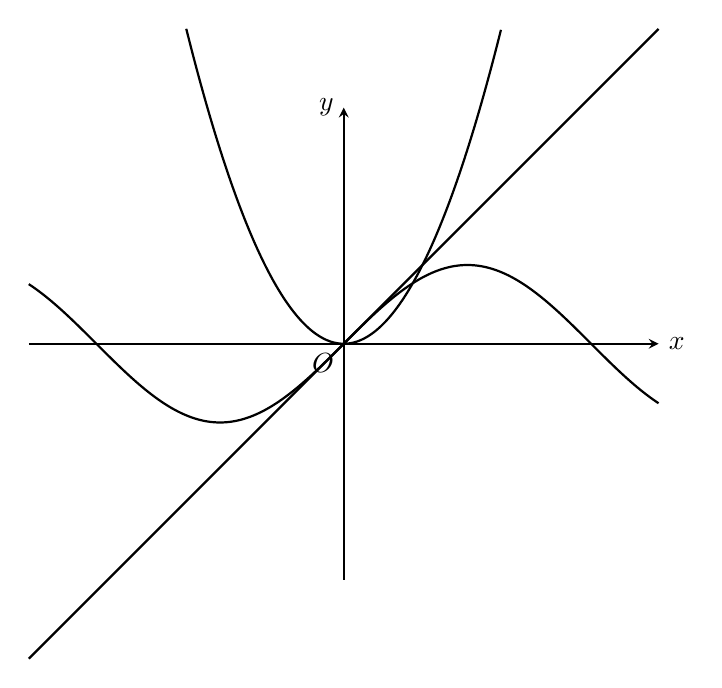
\begin{tikzpicture}[scale=1,samples=300]
        \draw[->,>=stealth,semithick] (-4,0)--(4,0) node[right]{$x$}; %x軸
        \draw[->,>=stealth,semithick] (0,-3)--(0,3) node[left]{$y$}; %y軸
        \draw (0,0) node[below left]{$O$}; %原点
        \draw[thick,domain=-4:4] plot(\x,{sin(\x r)});
        \draw[thick,domain=-2:2] plot(\x,{pow(\x,2)});
        \draw[thick,domain=-4:4] plot(\x,\x);
    \end{tikzpicture}
\end{tcblisting}

そこで \lstinlineiv{scope} 環境の \lstinlineiv{\clip} というコマンドを使ってグラフを切り取れば見やすいグラフになります．
\begin{tcblisting}{title=\texttt{scope} の \texttt{\textbackslash{}clip} で切り取る}
    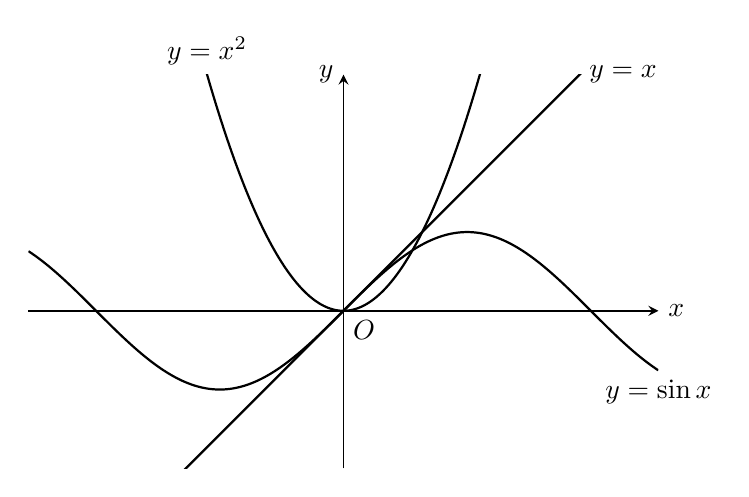
\begin{tikzpicture}[scale=1,samples=300]
        \draw[->,>=stealth,semithick] (-4,0)--(4,0) node[right]{$x$}; %x軸
        \draw[->,>=stealth,semithick] (0,-2)--(0,3) node[left]{$y$}; %y軸
        \draw (0,0) node[below right]{$O$}; %原点
        \begin{scope}
            \clip (-4,-2) rectangle(4,3);
            \draw[thick,domain=-4:4] plot(\x,{sin(\x r)});
            \draw[thick,domain=-2:2] plot(\x,{pow(\x,2)});
            \draw[thick,domain=-4:4] plot(\x,\x);
        \end{scope}
        \node[above] at ({-sqrt(3)},3) {$y=x^2$};
        \node[right] at (3,3) {$y=x$};
        \draw (4,{sin(4 r)}) node[below]{$y=\sin x$};
    \end{tikzpicture}
\end{tcblisting}
\lstinlineiv{node} や座標軸や，各グラフの式などは \lstinlineiv{scope} 環境の外に書かないと，切り取られてしまい描画されない可能性があります．

\end{document}
